\documentclass[class=book, crop=false, oneside, 12pt]{standalone}
\usepackage{standalone}
\usepackage{amsmath}
\usepackage{../../style}
\graphicspath{{./assets/images/}}

% arara: pdflatex: { synctex: yes, shell: yes }
% arara: latexmk: { clean: partial }
\begin{document}

\chapter{Forza elettrostatica. Campo elettrostatico}

\section{Cariche elettriche, isolanti e conduttori}

Tra le interazioni fondamentali esistenti in natura, la prima ad essere scoperta e studiata quantitativamente è stata l'interazione gravitazionale, responsabile di gran parte dei fenomeni che si osservano su scala macroscopica nell'universo.
Essa è dettata dalla legge:
\begin{equation}
    F = \gamma \frac{m_1 m_2}{r^2}
\end{equation}

Un'altra interazione fondamentale, che gioca un ruolo essenziale nella costituzione della materia, è quella elettromagnetica. 
Un aspetto particolare dell'interazione elettromagnetica è la forza elettrica.

Oggi noi attribuiamo le forze in parola a cariche elettriche, che sono preesistenti nei corpi e che passano da un corpo all'altro durante lo strofinio, per cui i corpi elettrizzati si chiamano anche elettricamente carichi.
Questi corpi che si caricano per strofinio sono detti \emph{isolanti}, in quanto capaci di trattenere la carica elettrica, mentre altri, come ad esempio i metalli e il corpo umano stesso, non trattengono la carica e sono detti \emph{conduttori}.

Sperimentalmente si deduce che esistono due diversi tipi di cariche elettriche; per convenzione è stata chiamata positiva la carica che compare sulla superficie delle sostanze tipo vetro quando vengono elettrizzate, mentre è stata chiamata negativa la carica che compare sulla superficie delle sostanze tipo bachelite.
Da questo ottengo i seguenti risultati:
\begin{itemize}
    \item due corpi isolanti carichi entrambi positivamente o entrambi negativamente si respingono; 
    \item un corpo isolante carico positivamente e uno carico negativamente si attraggono; 
    \item nel processo di carica per strofinio i due corpi, la bacchetta di isolante e il panno, acquistano sempre una carica di segno opposto. 
\end{itemize}

La carica che si accumula per strofinio sugli isolanti si mantiene per tempi considerevoli, specialmente se l'aria nell'ambiente in cui si opera è secca.  
Invece, come abbiamo già rilevato, non è possibile caricare per strofinio una bacchetta di metallo tenendola in mano, come si fa con le bacchette di isolante, a meno che non sia tenuta da una barretta di isolante, in tal caso si comporta in modo analogo.

L'assenza di elettrizzazione dei conduttori si spiega col fatto che i metalli e il corpo umano sono conduttori, cioè permettono il movimento della carica elettrica accumulatasi durante lo strofinio, a differenza di quanto avviene negli isolanti.
In questi esperimenti hanno caratteristiche di conduttori anche il suolo, svariati liquidi tra cui l'acqua e anche l'aria umida.

\section{Struttura elettrica della materia}

\subsection{Costituenti fondamentali}

La materia stabile che ci circonda (corpi terrestri, pianeti, la nostra galassia) è formata da tre costituenti elementari: il protone $p$, il neutrone $n$, l'elettrone $e$.

La massa del protone è circa eguale alla massa del neutrone e vale \(m_p \cong m_n \cong 1.67 \cdot 10^{-27} kg \); la massa dell'elettrone è \(m_e \cong 9.11 \cdot 10^{-31} kg\), circa 1840 volte più piccola della massa del protone e del neutrone.
Sulla base dei dati sperimentali esistenti il protone e il neutrone hanno dimensioni dell'ordine di \(10^{-15} m\).
Le dimensioni dell'elettrone sono inferiori a \(10^{-17} m\): esso ci appare puntiforme, cioè privo di struttura interna.

\subsection{Carica \emph{e}}

La carica elettrica dell'elettrone è la più piccola osservata sperimentalmente: essa è chiamata carica elementare ed è indicata con \(-e\); il segno evidenzia l'assunzione che la carica dell'elettrone sia negativa. 
Il protone ha una carica positiva \(+e\), eguale in valore assoluto a quella dell'elettrone, il neutrone invece ha carica elettrica nulla (è neutro).

La carica elettrica è una grandezza fisica \emph{quantizzata}, ossia la carica elettrica non varia con continuità ma ogni carica elettrica esistente in natura deve essere uguale o un multiplo intero della carica di un elettrone.

\subsection{Atomo}

I tre costituenti si aggregano in strutture che si chiamano atomi. 
In particolare un certo numero di protoni e neutroni, legati dall'interazione forte, costituiscono il nucleo dell'atomo, che risulta quindi carico positivamente; attorno al nucleo si muove un numero di elettroni, eguale al numero di protoni, sotto l'azione elettrica attrattiva esercitata dal nucleo. 
Poiché il numero di protoni in ogni atomo è eguale al numero di elettroni, la carica elettrica totale, somma delle singole cariche, è nulla e l'atomo è neutro.

\subsection{Carica di un isolante per strofinio}

Gli elettroni di un atomo, specialmente quelli periferici, sono più o meno legati al nucleo: da ciò deriva la differenza tra materiali isolanti e conduttori. \newline
Negli isolanti gli elettroni sono ben vincolati al nucleo e non possono spostarsi attraverso il corpo: gli isolanti non trasportano facilmente la carica. \newline
Mediante una specifica azione locale, quale lo strofinio con un panno, si può far passare, nei punti di contatto, un certo numero \(n\) di elettroni e quindi una carica \(-q = -ne\) da un corpo \(C_1\), ad esempio una bacchetta di vetro, ad un corpo \(C_2\), il panno; 
\(C_2\) risulta carico negativamente nei punti di contatto con \(C_1\) e tale carica non si muove verso altre zone di \(C_2\). 
Invece in \(C_1\) nei punti di contatto è presente un eccesso di carica positiva \(q = ne\). \newline
Nel caso di isolanti tipo bachelite il processo avviene in senso contrario. 

In conclusione un processo di carica per strofinio è un processo in cui vengono separate, attraverso un agente meccanico, delle cariche (elettroni) e trasferite da un corpo ad un altro. 
Lo spostamento riguarda un numero intero di elettroni, cioè la carica trasferita può assumere solo valori multipli interi della carica elementare, in accordo al fatto che la \emph{carica elettrica è quantizzata}.

\subsection{Principio di conservazione della carica elettrica}

In un sistema elettricamente isolato la somma algebrica di tutte le cariche elettriche rimane costante nel tempo, ovvero si conserva. 

\subsection{Ionizzazione}

Quando ad un atomo vengono aggiunti o tolti elettroni si forma rispettivamente uno ione negativo o uno ione positivo; in particolare il fenomeno di sottrazione di elettroni di chiama ionizzazione.

\section{La legge di Coulomb}

\subsection{Enunciato}

Coulomb stabilì che due cariche puntiformi \(q_1\) e \(q_2\), poste a distanza \(r\), interagiscono con una forza \(F\), diretta secondo la loro congiungente, di modulo
\begin{equation} \label{forza_coulomb}
    F = k \frac{q_1 q_2}{r^2}
\end{equation}
quindi \emph{la forza è direttamente proporzionale al prodotto delle cariche elettriche e inversamente proporzionale al quadrato della loro distanza.}

La costante \(k\) che compare in (\ref{forza_coulomb}) dipende dalla scelta delle unità di misura e dal mezzo in cui le cariche sono immerse, mezzo di norma isolante che per le sue proprietà elettriche viene chiamato \emph{dielettrico}. 

Come unità di carica si è definito il coulomb, simbolo \(C\), che è pari alla carica trasportata da una corrente di \(1 A\) in \(1\) secondo. \newline
Fissata l'unità di misura della carica, ed essendo già definite le unità di forza e di distanza, in linea di principio basta misurare la forza tra due cariche note a distanza nota per determinare nel sistema internazionale il valore di \(k\) nel vuoto; risulta
\begin{equation}
    k = 8.9875 \cdot 10^9 \frac{Nm^2}{C^2}
\end{equation}
La costante \(k\) può essere espressa anche come 
\begin{equation*}
    k = \frac{1}{4 \pi \epsilon_0}
\end{equation*}
dove la costante \(\epsilon_0\) è nota come costante dielettrica (o permittività) del vuoto e ha il valore
\begin{equation}
    \epsilon_0 = \frac{1}{4 \pi k} = 8.8542 \cdot 10^{-12} \frac{C^2}{N m^2}
\end{equation}
La legge di Coulomb si può esprimere quindi con
\begin{equation} \label{forza_coulomb_dielettica}
    F = \frac{1}{4 \pi \epsilon_0} \frac{q_1 q_2}{r^2}
\end{equation}
Il valore della carica elementare espresso in coulomb risulta 
\begin{equation}
    e = 1.6022 \cdot 10^{-19} C
\end{equation}

\subsection{Forza vettoriale della legge di Coulomb}

La legge (\ref{forza_coulomb_dielettica}) deve essere scritta in termini vettoriali, trattandosi dell'espressione di una forza.
La direzione della forza è quella della retta congiungente le due cariche puntiformi.

La forza che la carica \(q\) esercita sulla carica \(q_0\) assume la forma
\begin{equation}
    \overrightarrow{F} = \frac{1}{4 \pi \epsilon_0} \frac{q \ q_0}{r^2} \overrightarrow{u}
\end{equation}
Se \(q\) e \(q_0\) hanno lo stesso segno (\(q ,\ q_0 > 0\)), la forza ha lo stesso verso di \(\overrightarrow{u}\), è cioè \emph{repulsiva}; se invece \(q\) e \(q_0\) hanno segno opposto (\(q ,\ q_0 < 0\)) \(\overrightarrow{F}\) ha verso opposto ad \(\overrightarrow{u}\), è \emph{attrattiva}.

\section{Campo elettrostatico}

Le forze elettriche agenti su una carica \(q_0\) dovute alle cariche circostanti si sommano come vettori: vige cioè il principio di sovrapposizione, detto anche \emph{principio di indipendenza delle forze simultanee}.

La forza elettrostatica su una carica puntiforme \(q_0\), risultante delle forze esercitate da un sistema discreto di cariche puntiformi \(q_i\) è uguale a: 
\begin{equation}
    \overrightarrow{F} = \sum_i \overrightarrow{F}_i = \sum_i \frac{1}{4 \pi \epsilon_0} \frac{q_i \ q_0}{r^2} \overrightarrow{u}_i = q_0 \sum_i \frac{1}{4 \pi \epsilon_0} \frac{q_i}{r^2} \overrightarrow{u}_i  
\end{equation}

La grandezza vettoriale
\begin{equation}
    \overrightarrow{E} = \frac{\overrightarrow{F}}{q_0}
\end{equation}
viene chiamata \emph{campo elettrostatico} prodotto in un punto \(P\) da un sistema di cariche ferme che agiscono su \(q_0\).

\begin{figure}[h]
    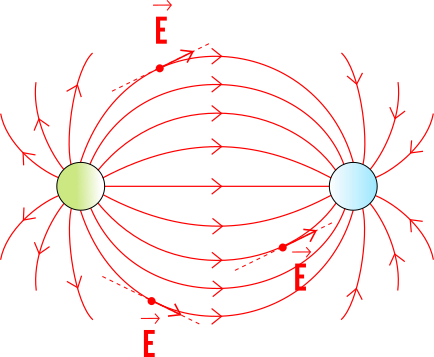
\includegraphics[scale=0.4]{campo-elettrico-linee-di-campo-elettrico}
    \centering
    \caption{Campo elettrostatico}
\end{figure}

Il campo elettrostatico generato da un sistema discreto di cariche puntiformi in un punto \(P\) è
\begin{equation}
    \overrightarrow{E} =\sum_i \frac{1}{4 \pi \epsilon_0} \frac{q_i}{r_i^2} \overrightarrow{u}_i
\end{equation}

Il campo elettrostatico in un punto \(P\) prodotto da un sistema discreto di cariche è uguale alle somma dei campi elettrostatici prodotti singolarmente dalla cariche.
\begin{equation} \label{equiv_campi}
    F ( x, y, z) = q_0 \ E ( x, y, z) 
\end{equation}

La (\ref{equiv_campi}) può essere interpretata dicendo che il sistema di cariche è la sorgente del campo elettrostatico \(E\): la carica \(q_0\) interagisce con questo subendo la forza \(F\); 
l'azione elettrica tra cariche, che è una azione a distanza, avviene attraverso il campo. 

\section{Campo elettrico prodotto da una distribuzione continua di cariche}

Se la distribuzione di carica è continua il campo elettrostatico che essa crea in un punto \(P\) si può ottenere dividendo, la carica in elementi infinitesimi \(dq\).  
Il campo elettrostatico prodotto da \(dq\) in un punto \(P\) distante \(r^{\prime}\) è approssimabile ad una carica puntiforme: 
\begin{equation*}
    d \overrightarrow{E} = \frac{d q}{4 \pi \epsilon_0 r^{\prime 2}} \overrightarrow{u}^{\prime}
\end{equation*}
Il campo elettrostatico risultante in \(P\) si calcola ricorrendo al principio di sovrapposizione; poiché la somma è estesa ad un numero infinito di contributi infinitesimi, essa si riduce ad un integrale vettoriale esteso a tutta la distribuzione continua:
\begin{equation}
    \overrightarrow{E} = \frac{1}{4 \pi \epsilon_0} \int \frac{dq}{r^{\prime 2}} \overrightarrow{u}_x
\end{equation}

Per chiarire il significato di questa formula (generale) si distinguono diversi casi caratterizzati da un elevato grado di simmetria.

\subsubsection*{Anello carico}

\begin{figure}[h]
    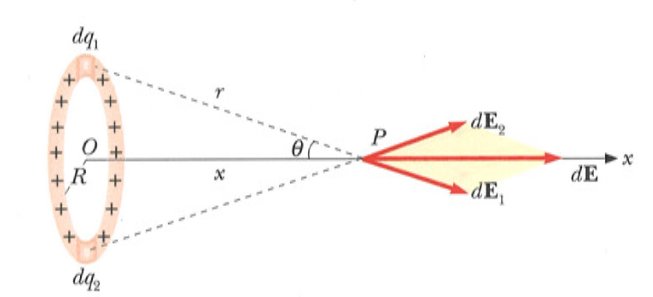
\includegraphics[scale=0.4]{anello_carico.png}
    \centering
    \caption{}
\end{figure}

Una carica \(q\) è distribuita uniformemente su un sottile anello di raggio \(R\).  
Il campo elettrico è dato dalla formula:
\begin{equation*}
    \overrightarrow{E} (x) = \frac{q}{4 \pi \epsilon_0} \frac{x}{\left(R^2 + x^2\right)^{3/2}} \overrightarrow{u}_x
\end{equation*}
con \(R\) raggio dell'anello, \(x\) la distanza dal punto \(P\).
Il campo elettrostatico è parallelo e concorde all'asse dell'anello per \(x > 0\), è parallelo e discorde per \(x < 0\) ed è nullo nel centro dell'anello, 
dove tutti i contributi elementari si elidono.

Nei punti a grande distanza dal centro (\(x >> R\)) 
\begin{equation*}
    \overrightarrow{E} (x>>R) =\frac{q}{4 \pi \epsilon_0 x^2} \overrightarrow{u}_x
\end{equation*}
concorde all'asse a destra e discorde a sinistra, come se la carica fosse concentrata nel centro dell'anello; non si distingue più, in questa situazione, la struttura della distribuzione.

\subsubsection*{Disco carico}

Un disco sottile di raggio \(R\) ha una carica \(q\) distribuita uniformemente su tutta la sua superficie.  
\begin{figure}[h]
    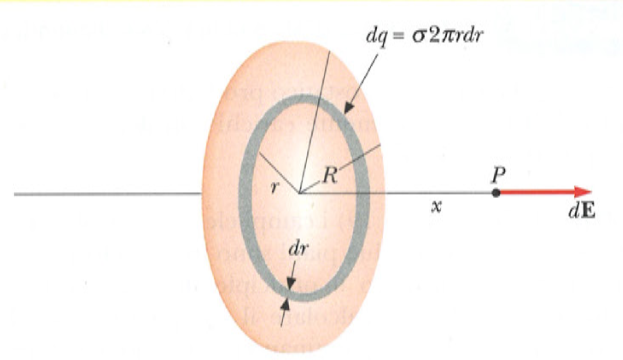
\includegraphics[scale=0.4]{disco_carico.png}
    \centering
    \caption{}
\end{figure}
Il campo elettrico è dato da:
\begin{equation*}
    \overrightarrow{E} (x) = \pm \frac{q}{2 \pi \epsilon_0 R^2} \left(1 - \frac{|x|}{\sqrt{x^2 + R^2}}\right) \overrightarrow{u}_x
\end{equation*}
Il segno positivo vale per \(x > 0\), quello negativo per \(x < 0\).  
Anche in questo caso, ad una lunga distanza, il disco è visto come carica puntiforme.  

Quando x tende a zero i limiti destro e sinistro del campo sono diversi e valgono rispettivamente
\begin{equation*}
    \overrightarrow{E}_{+} (x) = \frac{\sigma}{2 \epsilon_0} \overrightarrow{u}_x \ , \ \overrightarrow{E}_{-} (x) = - \frac{\sigma}{2 \epsilon_0} \overrightarrow{u}_x 
\end{equation*}

Se ora facciamo tendere \(R\) all'infinito, mantenendo \(\sigma\) costante, otteniamo un piano indefinito uniformemente carico
\begin{equation*}
    E = \pm \frac{\sigma}{2 \epsilon_0} \overrightarrow{u}_x
\end{equation*}
ed è ortogonale al piano, uscente da esso e costante in ogni punto dello spazio, anche detto \emph{uniforme}.

\begin{figure}[h]
    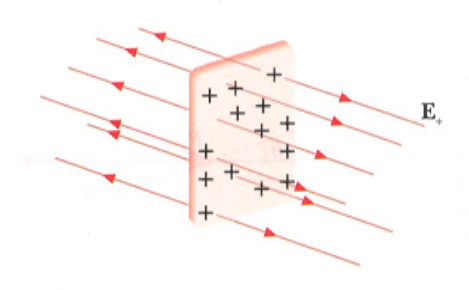
\includegraphics[scale=0.4]{piano_carico1.png}
    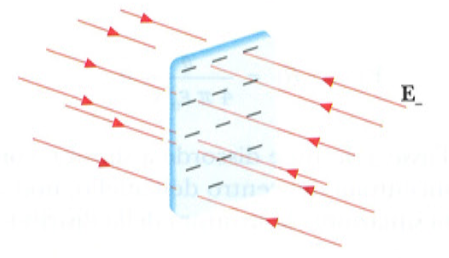
\includegraphics[scale=0.4]{piano_carico2.png}
    \centering
    \caption{}
\end{figure}

\subsubsection*{Due piani indefiniti carichi}

Dati due piani indefiniti carichi con densità superficiale l'uno \(+ \sigma\) e l'altro \(- \sigma\).
i campi elettrostatici \(\overrightarrow{E}_{+}\) e \(\overrightarrow{E}_{-}\) generati separatamente dai due piani sono in modulo entrambi eguali a \(\sigma / 2 \epsilon_0\).
Utilizzando il principio di sovrapposizione, per calcolare il campo risultante \(\overrightarrow{E} = \overrightarrow{E}_{+} + \overrightarrow{E}_{-}\) si vede che i campi si sommano nella regione compresa tra i due piani e si annullano all'esterno.  
All'interno il campo elettrico vale:
\begin{equation*}
    \overrightarrow{E} = \frac{\sigma}{\epsilon_0} \overrightarrow{u}_x
\end{equation*}
nullo all'esterno dei due piani.
\begin{figure}[h]
    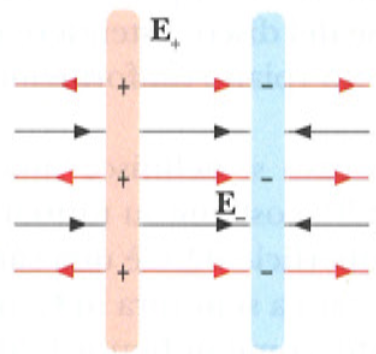
\includegraphics[scale=0.4]{piani_carichi1.png}
    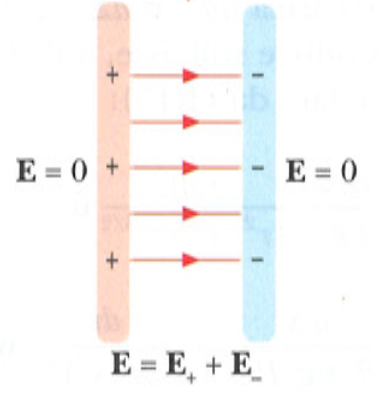
\includegraphics[scale=0.4]{piani_carichi2.png}
    \centering
    \caption{}
\end{figure}
Una caratteristica comune degli esempi mostrati è che le distribuzioni di carica sono \emph{uniformi}.

\section{Linee di forza del campo elettrostatico}
L'introduzione del concetto di campo elettrostatico mette in evidenza che la presenza di un sistema di cariche, dal caso più semplice della singola carica puntiforme al caso più generale di una distribuzione spaziale, modifica lo spazio circostante nel senso che una carica di prova posta in un qualsiasi punto risente della forza (\ref{equiv_campi}), attribuita all'interazione con il campo elettrostatico.

Partendo da una generica posizione e muovendosi per tratti infinitesimi successivi, ciascuno parallelo e concorde al campo elettrostatico in quel dato punto, si ottiene una linea che è detta \emph{linea di forza} o \emph{linea del campo elettrostatico}: 
pertanto in ogni suo punto tale linea per definizione è tangente al campo e il suo verso di percorrenza indica il verso del campo.

Nel caso di una carica puntiforme, le linee di forza hanno direzione radiale con origine sulla carica e sono uscenti da questa se è positiva, entranti se è negativa. 
Le linee si infittiscono man mano che ci si avvicina alla sorgente del campo e ciò indica che l'intensità del campo è crescente. 

Le proprietà delle linee di forza sono quindi:
\begin{itemize}
    \item una linea di forza in ogni suo punto è tangente e concorde al campo elettrostatico in quel punto;
    \item le linee di forza si addensano dove l'intensità del campo elettrostatico è maggiore; 
    \item le linee di forza non si incrociano mai, in quanto in ogni punto il campo elettrostatico è definito univocamente e non può avere due direzioni distinte;
    \item le linee di forza hanno origine dalle cariche positive e terminano sulle cariche negative; qualora ci siano solo cariche di uno stesso segno le linee di forza si chiudono all'infinito.
\end{itemize}

\begin{figure}[h]
    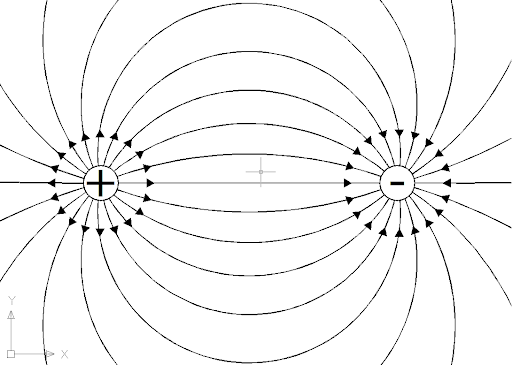
\includegraphics[scale=0.4]{linee-di-forza}
    \centering
    \caption{Linee di forza}
\end{figure}

Nel caso di cariche di segno opposto, ma eguali in modulo, tutte le linee che partono dalle cariche positive si chiudono su quelle negative, alcune passando eventualmente per l'infinito; 
se le cariche sono dello stesso segno, come in, tutte le linee che provengono dalle cariche si chiudono all'infinito; 
se invece le cariche non sono eguali in modulo, alcune linee terminano o provengono dall'infinito.

\begin{figure}[h]
    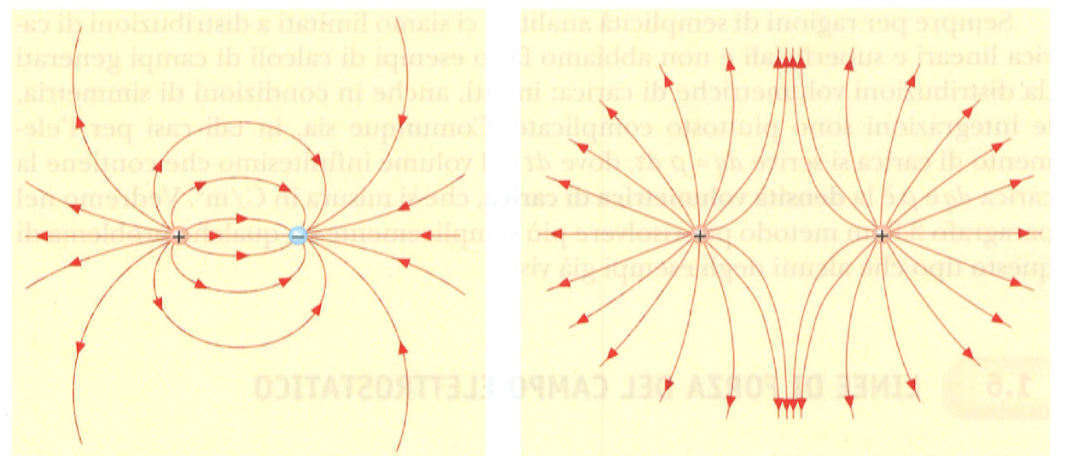
\includegraphics[scale=0.4]{linee_infinito.png}
    \centering
    \caption{Linee di forza}
\end{figure}

\section{Moto di una carica in un campo elettrostatico}

Supponiamo di immettere una carica \(q\) di piccole dimensioni, puntiforme, in una zona di spazio in cui esiste un campo elettrostatico generato da un sistema di cariche ferme, che non vengono perturbate in alcun modo dalla presenza della carica. 
Questa, di massa \(m\), è sottoposta alla forza (\ref{equiv_campi}) e la legge della dinamica di Newton, in condizioni non relativistiche, si scrive
\begin{equation}
    q \overrightarrow{E} = m \overrightarrow{a} \implies \overrightarrow{a} = \frac{q}{m} \overrightarrow{E}
\end{equation}
Integrando si determinano posizione e velocità della carica, note posizione e velocità iniziali. 

Se \(\overrightarrow{E}\) è uniforme (costante in modulo e in direzione), l'accelerazione \(\overrightarrow{a}\) è una costante del moto. 
Se la carica \(q\) è positiva, l'accelerazione sarà nel verso di \(\overrightarrow{E}\), se la carica \(q\) è negativa sarà nel verso opposto.

\end{document}